% ======================================================================================
% CLUSTERING
%
% graphs to insert:
%	- score vs silhouette coefficient per cluster
%	- sample silhouette values for the best number of clusters
%	- 3D/2D cluster representation for the best number of clusters
% tables to insert:
%	- PCA outcome of the features
%	- object to cluster assignment depending on number of clusters (the best ones)
%	- cluster sizes depending on number of clusters
% figures:
%	- mean values of the features per cluster applied to the object


\section{Clustering}
Here we report the results from clustering depending on different features used.

%\begin{figure}
	%\centering
	%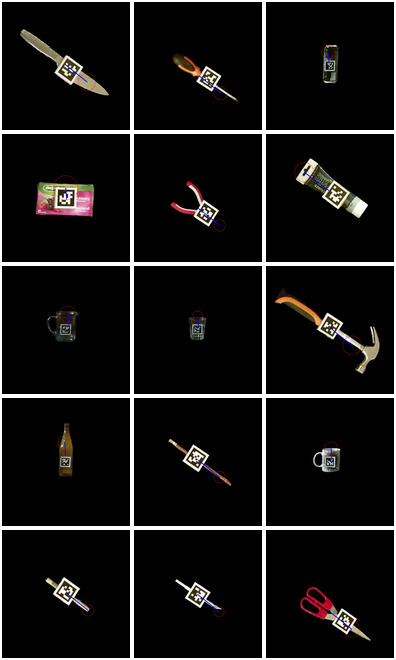
\includegraphics[width=\textwidth]{img/results/object_handovers.jpg}
	%\caption{Resulting handover data applied to each object}
	%\label{fig:object_handovers}
%\end{figure}


\subsection{Principal Component Analysis}


\subsection{K-means}

\input{tex/plot_scores.tex}

\input{tex/plot_silhouette_5.tex}

\input{tex/plot_silhouette_6.tex}

\input{tex/plot_silhouette_7.tex}

\input{tex/plot_clusters.tex}

\subsection{Object cluster assignments}



% ======================================================================================
% CLASSIFICATION
%
% GRAPHS:
%	- loss per step
%	- accuracy per step (validation and testing)
%	- training speed
% TABLES:
%	- confusion matrix
%	- accuracy per object
%	-

\section{Classification}
Output different results from classification depending on which layers are trained further and network architecture.

